\chapter{Implementación}
En este capítulo se mencionarán tecnologías usadas, así como las estructura del proyecto, diseños usados etc.\\[6pt]
El lenguaje de programación utilizado para la realización del proyecto ha sido \textbf{Python}~\cite{VanRossum2009}, concretamente la versión $3.10.12$. Librerías tales como \textbf{scikit-learn}~\cite{scikit-learn}, \textbf{matplotlib}~\cite{Hunter2007}, \textbf{numpy}~\cite{harris2020array} y \textbf{pandas}~\cite{reback2020pandas} han sido imprescindibles para el desarrollo del proyecto. Junto a estos paquetes, se han usado otros secundarios para facilitar el desarrollo.\\[6pt]
La colección completa de algoritmos en su versión original (a excepción de modificaciones del \textbf{GA} y el algoritmo completo de \textbf{ACO}) han sido obtenidos del repositorio \textbf{PyMetaheuristics}~\cite{valdecy_pyMetaheuristic}.\\[6pt]
La estructura del proyecto, junto con los scripts principales, es la siguiente:

\begin{itemize}
    \item \texttt{data} -- Almacena los conjuntos de datos utilizados por el proyecto.
    \item \texttt{docs} -- Documentación relacionada con el proyecto en latex.
    \item \texttt{img} -- Imágenes generadas en el proyecto.
    \item \texttt{LICENSE} -- Términos de distribución del proyecto.
    \item \texttt{README.md} -- Descripción general.
    \item \texttt{requirements.txt} -- Dependencias del proyecto.
    \item \texttt{results} -- Resultados generados por el proyecto (fitness, tiempos, etc.).
    \item \texttt{scripts} -- Scripts y programas secundarios en bash.
    \item \texttt{src} -- Código fuente del proyecto.
    \item \texttt{utils} -- Módulos y scripts de utilidad.
    \item \texttt{venv} -- Entorno virtual de Python.
\end{itemize}

El repositorio ha sido almacenado en la plataforma \textbf{Github} desde el comienzo del proyecto. De forma obvia, la herramienta usada para el control del versiones es \textbf{Git}~\cite{chacon2014pro}. Se muestra una gráfica con los commits realizados durante todo el desarrollo del proyecto en \ref{fig:commits}

\begin{figure}[htp]
    \centering
    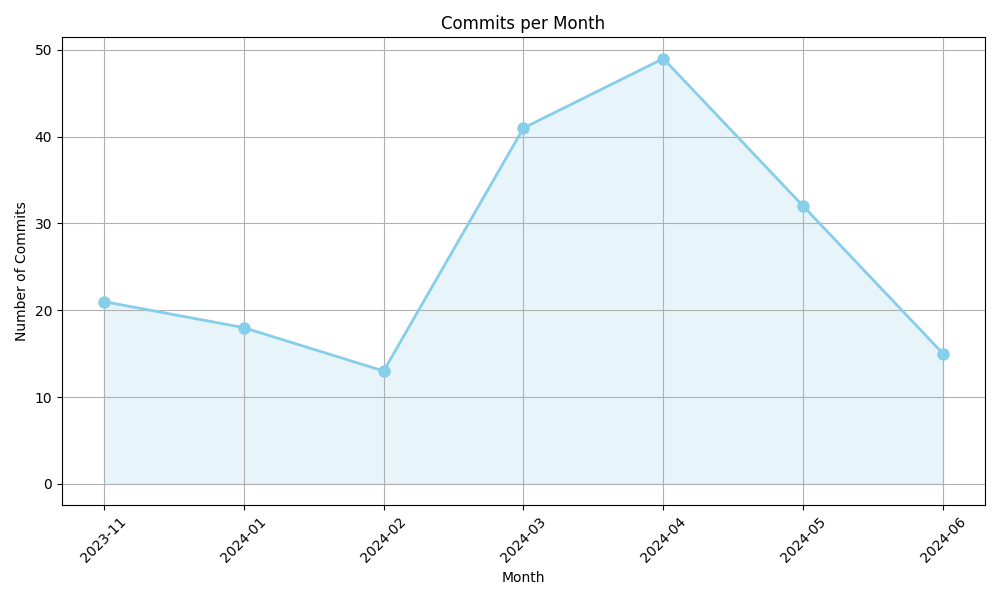
\includegraphics[width=1\textwidth]{imagenes/commits_chart.png}
    \caption{Comits realizados durante todo el proyecto}
    \label{fig:commits}
\end{figure}

Durante el desarrollo del software se utilizó el patrón de diseño \textit{Strategy} o estrategia~\cite{refactoring-guru-strategy}. Es un patrón de diseño de software que pertenece al grupo de patrones de comportamiento. Su objetivo principal es definir una familia de algoritmos, encapsular cada uno de ellos y hacerlos intercambiables. Esto permite que el algoritmo pueda variar independientemente del problema a optimizar. Se crea pues la clase \textit{Optimizer} \ref{fig:optimizer_class} siguiendo este patrón.

\begin{figure}[htp]
    \centering
    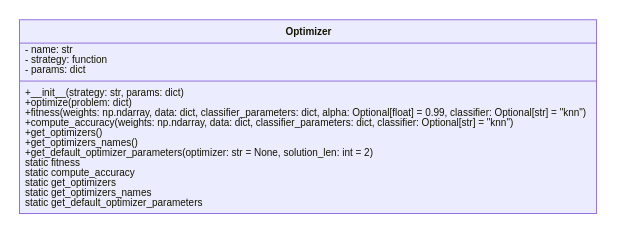
\includegraphics[width=1.2\textwidth]{imagenes/mermaid-diagram-20240616183528.png}
    \caption{Clase \textit{Optimizer} - patrón \textit{Strategy}}
    \label{fig:optimizer_class}
\end{figure}

De esta forma, a la hora de optimizar cualquier conjunto de datos, basta con llamar a un optimizador y especificar la metaheurística junto a su configuración, aunque existe una por defecto para cada ``estrategia''.\\[6pt]
Para mayor información y revisión del código utilizado en el proyecto, se refiere al lector al siguiente enlace: \url{https://github.com/Migue8gl/TFG-Wrapper-Based-Metaheuristics-Feature-Selection}.